\section{App Backup}

Para lidar com o caso de indisponibilidade do controlador local Morpheus, da rede local (roteador wireless) ou da conexão com a Internet, foi desenvolvido um aplicativo de \textit{backup}. Esse aplicativo permite acesso direto ao módulo, através do endereço local (supondo que o dispositivo celular esteja na mesma rede) ou por conexão direta com o ponto de acesso do módulo (disponível todo o tempo, ou sempre que o módulo não consiga conexão com a internet, a depender da preferência do usuário).

\subsection{Navegação}

A partir da tela inicial, um cliente pode verificar todos os módulos presentes em sua casa, visualizar temperatura, umidade, luminosidade, sensores de presença ou abertura e apagar ou acender luzes (para atuadores protegidos com senha, o usuário deve acessar a página do respectivo módulo), numa interface configurável (o usuário pode configurar quais parâmetros observar nesse menu principal). A exibição da Figura \ref{fig:telasPrincipaisBackup} é própria para celulares, enquanto a exibição da Figura \ref{fig:plantaBackup}, com posicionamento configurável, simula a planta de uma casa (num cenário real, poderia ser a própria planta da casa do usuário), e é própria para desktops.

\begin{figure}[H]
	\centering
	\caption{Telas principais do aplicativo backup}
  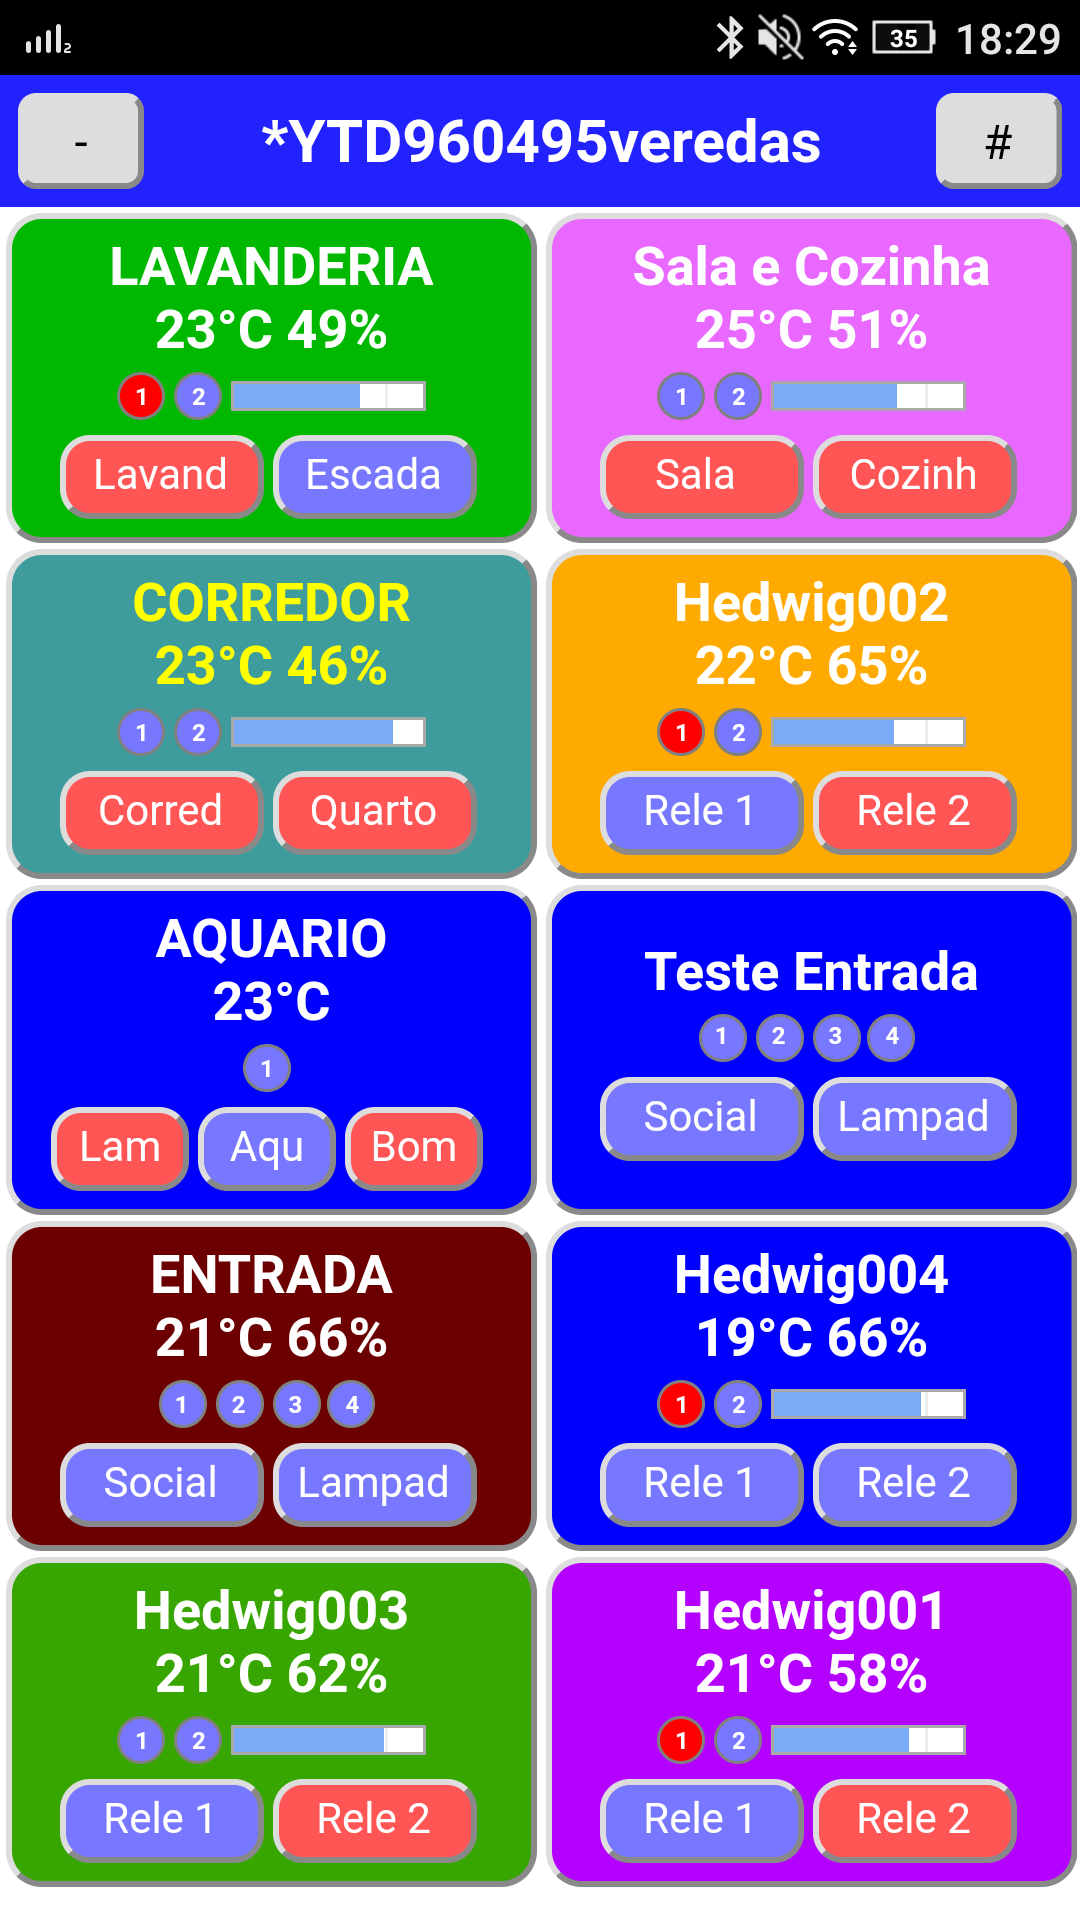
\includegraphics[width=0.5\textwidth]{telasPrincipaisBackup}
\label{fig:telasPrincipaisBackup}
\end{figure}

\begin{figure}[H]
  \centering
  \caption{Visão geral de uma planta com o aplicativo backup}
  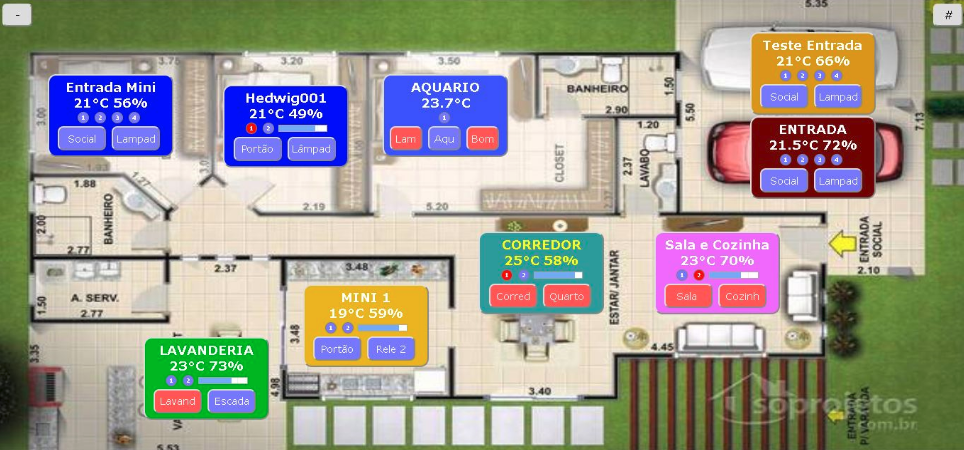
\includegraphics[width=0.8\textwidth]{plantaBackup}
  \label{fig:plantaBackup}
\end{figure}

A partir do menu principal, podemos acessar o menu do módulo desejado (vide Figura \ref{fig:menuPrincipalBackup}). Nele, encontram-se informações de luminosidade, horário, data, temperatura, umidade, sensor de presença (sensor 1) e sensor de abertura (sensor 2), além de controle de portão,lâmpada ou eletrodoméstico. Também exibe o nível de WiFi do módulo e a versão do firmware.

\begin{figure}[hbp]
    \centering
    \begin{minipage}{.4\linewidth}
        \centering
        \captionof{figure}{Menu Principal}
        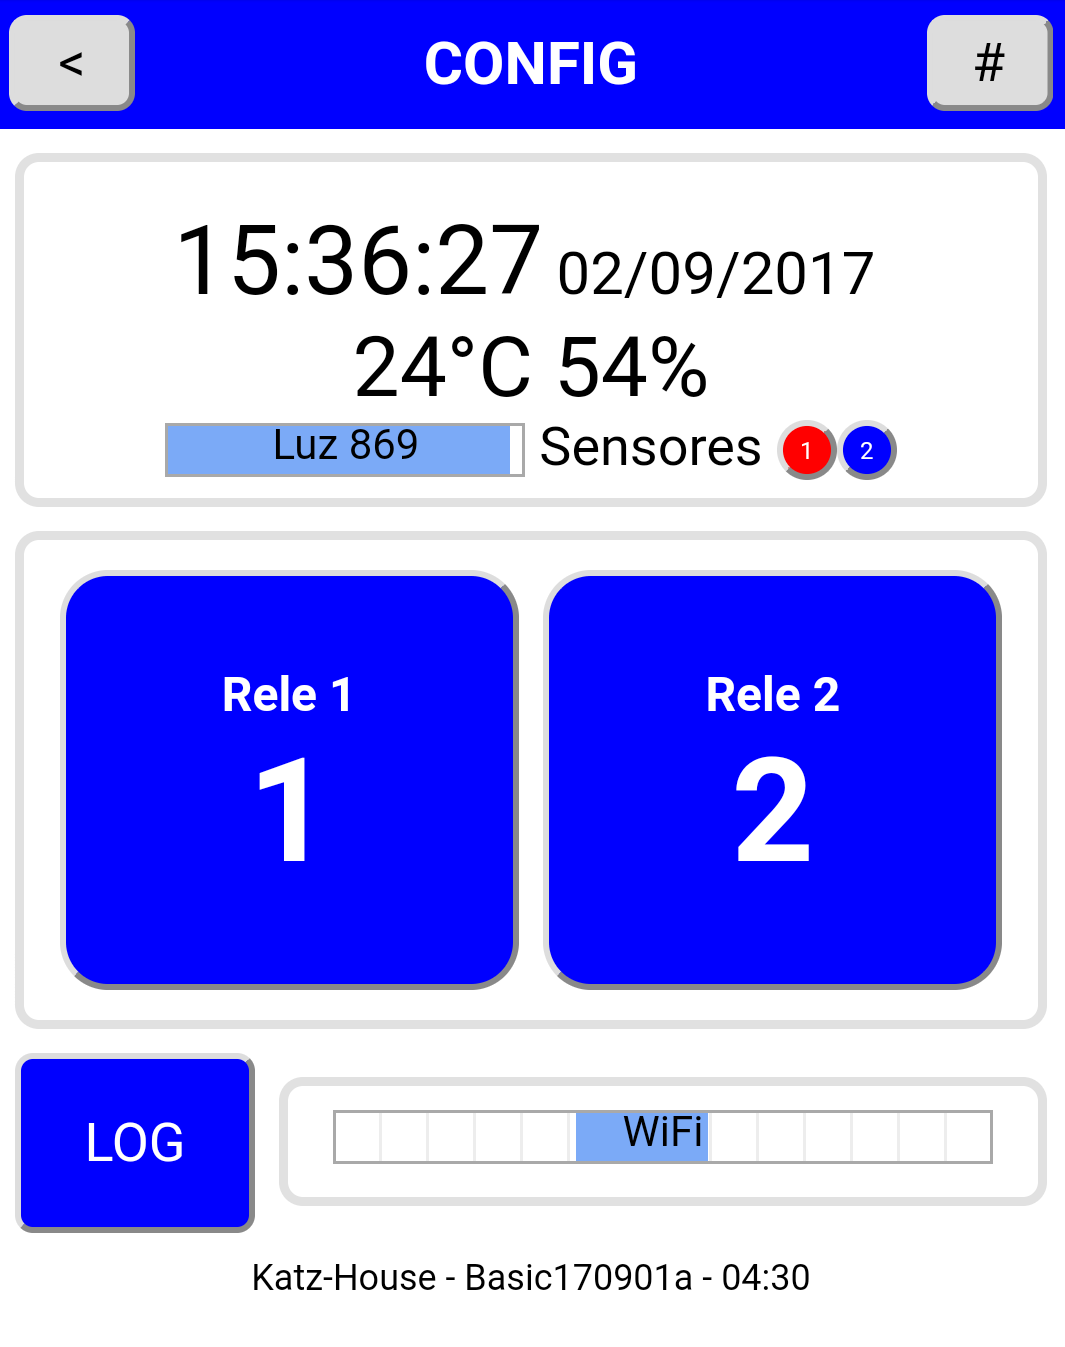
\includegraphics[height=6cm]{menuPrincipalBackup}
        \label{fig:menuPrincipalBackup}
    \end{minipage}
    \hfill
    \begin{minipage}{.4\linewidth}
        \centering
        \captionof{figure}{Teclado para digitação da senha}
        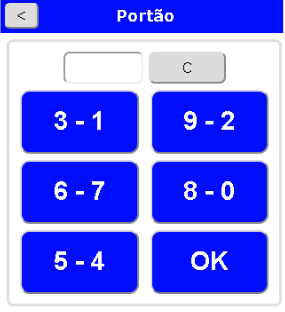
\includegraphics[height=6cm]{senhaBackup}
        \label{fig:senhaBackup}
    \end{minipage}
\end{figure}

No caso de proteção de controle por senha, é exibido o painel numérico como na Figura \ref{fig:senhaBackup}. A cada requisição da página, o modulo manda um mapeamento das teclas diferente (por exemplo, de teclas A,B,C,... para (3,1), (9,2), ...). Após o usuário entrar com a senha (sequência de teclas do tipo A, B, C, …), o módulo valida a sequência e autoriza o acionamento. Dessa forma, pessoas não conseguem copiar a senha ao visualizar a sequência de teclas do usuário, tampouco um invasor poderia copiar a sequência e utilizá-la para abertura logo em seguida, pois o mapeamento seria outro.

\subsection{Configurações}

A partir do menu principal do módulo, pode-se ter acesso ao seu log (para depuração, opção apenas para administradores) e um menu de configurações. Do menu de configurações, pode-se alterar o modo do display (dentre 3 opções), e as cores do módulo, conforme opções anteriormente citadas.

Ainda do menu de configurações, pode-se configurar alertas e alarmes (sonoros a partir dos módulos, e pela internet através do provedor gratuito Blynk e e-mail), relés (possibilidade de auto ligar a partir de um sensor específico, ou de ser acionado a partir de um sinal de rádio - usualmente um controle remoto ou até um sensor de abertura adicional, ou mais de um), e o log (quais parâmetros serão persistidos e mandados para a nuvem). Também pode-se acessar o menu de Ferramentas, onde é possível realizar testes de auto reset (para verificação do funcionamento do circuito antitravamento, que age em cerca de 30 segundos), reiniciar o módulo, desconectá-lo, voltar à versão de fábrica (versão implementada em software, enquanto a versão em hardware é realizada por meio de botão oculto), e atualizar o firmware (apenas disponível para administradores).
Ao acessar a atualização de firmware, escolhe-se a opção, que mostra a versão atual e, após escolha do arquivo, a versão a ser inserida.

% TODO era pra essa tela ao centro citada na linha abaixo estar em algum lugar?
É possível, também, acessar as configurações avançadas (tela ao centro). Nela, podemos configurar um offset para temperatura e umidade (de preferência realizados a partir de um medidor confiável para calibração).

Do menu de configurações avançadas, podemos configurar os sensores e controladores de radio frequência (sem fio), aspectos de conectividade do servidor gratuito Blynk e possivelmente trocar a rede WiFi em que o módulo está conectado. Ainda, para administradores, há a opção de configurar os usuários que têm acesso ao módulo.

Ainda pode-se trocar o nome do módulo, e ativar/desativar o ponto de acesso (para acesso direto ao módulo), além de configurar o nome (SSID) e senha de sua rede WiFi.

Demais ilustrações, referentes às configurações, estão disponíveis no Anexo \ref{attachmentsImagensBackup}{}.

\subsection{Abertura de porta do roteador}

% TODO importante explicar melhor que porta é essa que está sendo aberta, e por que

Para acessar o módulo/menu remotamente, podemos usar a abertura de porta (NAT/virtual servers), configurável nas páginas de configuração dos roteadores. Maiores informações para essa configuração podem ser encontradas nos manuais dos roteadores. (Observe que há uma segurança menor envolvida com essa configuração).

\begin{figure}[hbp]
    \centering
    \caption{Página de configuração TP Link}
    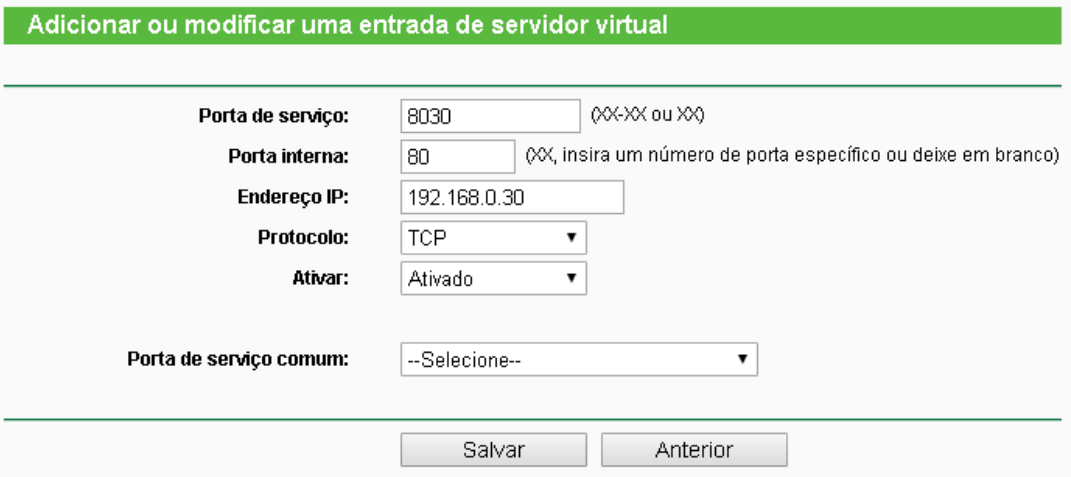
\includegraphics[width=0.8\textwidth]{tpLinkAppBackup}
    \label{fig:plantaBackup}
\end{figure}

\emph{Obs.:} Caso sua operadora só forneça o CGNAT, a abertura de porta por parte do usuário não será possível.

\subsection{Controle remoto}

Para que o controle remoto seja corretamente configurado, são necessários os seguintes passos.
\begin{enumerate}
    \item
    A partir da página inicial do módulo, entre em \# \textrightarrow{} Configurações Avançadas \textrightarrow{} RF433

    \item
    Configure o Sensor de Abertura “Sulton” no modo 2, para mandar sinais diferentes de abertura e fechamento. Consulte o manual do fabricante.

    \item
    Aperte +, espere até a página indicar “Aguardando”, e abra o sensor de abertura. (Podemos incluir diversos sinais para o controle do mesmo relé, abertura ou fechamento de sensor). Aperte “OK” no canto superior direito da página, para salvar suas configurações.

    \item
    Repita o passo 3 para o fechamento do sensor de abertura. \textbf{Cuidado:} O sensor de abertura repete algumas vezes o mesmo sinal. Aguarde alguns instantes entre gravar a abertura e o fechamento para não gravar o mesmo sinal (isso pode ser verificado na série numérica que aparece gravada. Se estiver igual, temos um problema).

    \item
        \begin{enumerate}
            \item
            A partir da página inicial do módulo, entre em \# \textrightarrow{} Configurações Avançadas \textrightarrow{} RF433.

            \item
            Aperte + (ao lado do rele 1 ou rele 2), espere até a página indicar “Aguardando”, e abra o sensor de abertura. (Podemos incluir diversos sinais para o controle do mesmo relé, abertura ou fechamento de sensor).

            \item
            Aperte "OK" no canto superior direito da página, para salvar suas configurações.

        \end{enumerate}
\end{enumerate}

\subsection{Notificações}
Para que as notificações sejam ativadas, utilize os próximos passos.

\begin{enumerate}
    \item
    Para que o suporte consiga acessar remotamente o módulo e realize a coleta de dados, acesse \# \textrightarrow{} Configurações Avançadas.\textrightarrow{} Blynk

    \item
    Insira o Auth Token (e.g. aa7a6dc1170640f08e951ed8cd2198a1).

    \item
    Selecione Notificações ao iniciar: Sim, e WiFi: Sim.

    \item
    Aperte em OK, no canto superior direito, para salvar suas alterações.
\end{enumerate}

\subsection{Offset Temperatura e Umidade}

\begin{enumerate}
    \item
    Para que o suporte consiga acessar remotamente o módulo e realize a coleta de dados, acesse \# \textrightarrow{} Configurações Avançadas.\textrightarrow{} Temperatura e Umidade.

    \item
    Efetue a calibração do equipamento usando uma referência externa.

    \item
    Aperte em OK, no canto superior direito, para salvar suas alterações.
\end{enumerate}

% \subsection{Serviços essenciais}
